\documentclass[tikz,fontsize=8pt]{standalone}
\usepackage{fourier}
\usetikzlibrary{arrows.meta}
\usetikzlibrary{calc}
\tikzset{>=latex}
\definecolor{bookblue}{RGB}{0,173,239}
\definecolor{bookpink}{RGB}{236,0,140}
\definecolor{bookgreen}{RGB}{50,200,0}
\definecolor{bookbluearea}{RGB}{204,239,252}
\tikzstyle{blueline}=[draw=bookblue,line width=0.2mm]
\tikzstyle{pinkline}=[draw=bookpink,line width=0.2mm]
\tikzstyle{greenline}=[draw=bookgreen,line width=0.2mm]
\tikzstyle{blackline}=[draw=black,line width=0.2mm]
\tikzstyle{bluearea}=[fill=bookbluearea]

\usepackage{scrextend}
\usepackage[utf8]{inputenc}
\changefontsizes[8pt]{8pt}
\usetikzlibrary{decorations.pathreplacing}
\begin{document}
  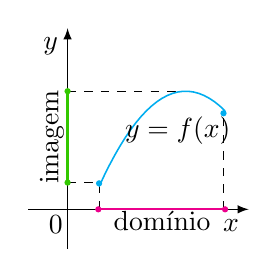
\begin{tikzpicture}
    \node at (-0.15,-0.2) {0};
    \draw[->] (-0.5,0) -- (2.3,0) node[below left] {$x$};
    \draw[->] (0,-0.5) -- (0,2.3) node[below left] {$y$};
    
    % Pink line, points and dashes
    \draw[pinkline,thick] (0.4,0) -- (2,0);
    \draw [dashed, line width=0.15mm] (0.4,0) -- (0.4,0.3);
    \draw [dashed, line width=0.15mm] (1.98,0) -- (1.98,1.28);
    \fill[bookpink] (0.39,0) circle (0.4mm);
    \fill[bookpink] (2,0) circle (0.4mm);
    
    % Green line, points and dashes
    \draw[greenline,thick] (0,0.34) -- (0,1.5);
    \draw [dashed, line width=0.15mm] (0,0.34) -- (0.4,0.34);
    \draw [dashed, line width=0.15mm] (0,1.5) -- (1.58,1.5);
    \fill[bookgreen] (0,0.34) circle (0.4mm);
    \fill[bookgreen] (0,1.5) circle (0.4mm);

    % Blue curve and points
    \fill[bookblue] (0.4,0.33) circle (0.4mm);
    \fill[bookblue] (1.98,1.22) circle (0.4mm);
    \draw[blueline,domain=-1.1:0.5] plot (\x+1.5,{-(\x)^2+1.5});
    

    \node[rotate=90] at (-0.2,0.92) {imagem};
    \node at (1.4,1) {$y=f(x)$};
    %\draw [decorate,decoration={brace,mirror},xshift=-4pt,yshift=0pt]
    %(0.85,0.78) -- (1.88,0.78) node [black,midway,yshift=-0.3cm] 
    %{\footnotesize $x-a$};
    %\draw [decorate,decoration={brace,mirror},xshift=-4pt,yshift=0pt]
    %(1.95,0.83) -- (1.95,1.38) node [black,midway,xshift=0.65cm] 
    %{\footnotesize $f(x)-f(a)$};
    %\draw[greenline] (0.7,0.83) -- (1.78,0.83);
    %\draw[greenline] (1.78,0.83) -- (1.78,1.43);
    %\draw[blueline]  (-0.3,0.3) -- (2.3,1.7);
    
    \node at (1.2,-0.15) {domínio};
  \end{tikzpicture}
\end{document}